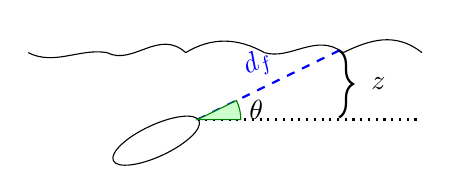
\begin{tikzpicture}
%Water surface
\draw (0,0) .. controls (0.33,-0.17) and (0.66,0.06) .. (1,0);
\draw (1,0) .. controls (1.33,-0.17) and (1.66,0.31) .. (2,0);
\draw (2,0) .. controls (2.33,0.2) and (2.66,0.19) .. (3,0);
\draw (3,0) .. controls (3.33,-0.1) and (3.66,0.26) .. (4,0);
\draw (4,0) .. controls (4.33,0.16) and (4.66,0.27) .. (5,0);

%AUV
\draw[rotate=25] (1,-1.7) ellipse (0.6 and 0.2);

%Aux
\draw[dashed, thick, blue] (2.15,-0.85) -- ++(26:2) node[midway, above, rotate=25]{$d_f$};
\draw[dotted, thick] (2.15,-0.85) -- (5,-0.85);
%Angles
\filldraw[fill=green!20,draw=green!50!black] (2.15,-0.85) -- ++(0.55,0) arc (0:26:0.55) node[midway, right] {$\theta$} -- cycle; 

%Curli braces
\path (2.15,-0.85)++(26:2) coordinate (water); 
\draw [decorate, decoration={brace, amplitude=5pt, mirror}, thick] (water)++(0,-0.85)  -- (water)
 node[label, midway, xshift=5mm] {$z$};

\end{tikzpicture}